\chapter{Imaging the Extended Groth Strip with the full LOFAR array}\label{section.EGS.hires}
\minitoc
\section{Aims \& Methodology}

\pg
Having made both a wide-field image of the EGS without international stations and a high-resolution model of the brightest source in the LOFAR primary beam, 3C295, in order to calibrate the international LOFAR station, we can now begin to proceed to imaging the EGS with the international LOFAR stations.
Before we do so, however, we must quantify whether the direction-independent calibration on the international baselines is sufficient when imaging the EGS. We expect to see some direction-dependent effects arising in the neighbourhood of 3C295: are these direction-dependent effect so severe that it is not worth imaging the EGS?



\pg
In other words, we seek to estimate whether, in practice, the EGS can, in part or in full, be placed on the same facet as 3C295 - and with what loss in accuracy to directional gain errors. The first direction-dependent effect we must take into account is decorrelation, also known as smearing (see \cref{section.RIME.TimeDep}). This effect causes signal loss on the longest baselines for sources far from the phase centre. A significant preliminary test is therefore to check that we do in fact see any of the LBCS sources - which we do, as will be demonstrated fully below. However, this is not the end of the problem: decorrelation causes flux from a source to be ``smeared" (hence its other name) around the source. The DDFacet suite can account for this effect by modelling the direction-dependent PSF, i.e. a PSF which is smeared appropriately as a function of position\footnote{A single smeared PSF is calculated per facet, and this smeared PSF is treated as being constant within the facet: this is a good approximation unless one uses truly massive facets.}

\begin{figure}[h!]
\centering
\begin{subfigure}{.48\textwidth}
\resizebox{\hsize}{!}{\includegraphics{images/{MSlist.fullBW.LOBOS1.MSlist.fullBW.txt.uniform.psf.fits}.png}}
\caption{\label{image.ddPSF.1} Direction-dependent PSF near LBCS1}
\end{subfigure}
\hfill
\begin{subfigure}{.48\textwidth}
\resizebox{\hsize}{!}{\includegraphics{images/{MSlist.fullBW.LOBOS6.MSlist.fullBW.txt.uniform.psf.fits}.png}}
\caption{\label{image.ddPSF.2} Direction-dependent PSF near LBCS6}
\end{subfigure}
\caption{\label{image.ddPSF} Cutouts showing the direction-dependent PSF at two different points in the primary beam of our observation.}
\end{figure}

\pg
The second source of direction-dependent effects is physical: the signal from different parts of the sky propagates through different parts of the local ionosphere before reaching our antennas. In the ideal case, our direction-independent calibration of the EGS using 3C295 as a calibrator is good enough, for international baselines, to allow the imaging of the full EGS using international LOFAR, with acceptable upper bounds to decorrelation throughout the field. Of course, this is unlikely to be the case - the aim is then to find out just how far we are from this ideal scenario.

\pg
In RIME terms, when performing our direction-independent calibration, we solved for $\hatJones_{3C295,p}^{t,\nu}$ (see \cref{3c295.dirin.cal}), assuming that it was the dominant source of signal in the sky. By applying the inverse of this gain solution to the visibilities, we image the \textit{corrected visibilities}:
\begin{align}
\Vis_{pq}^\mathrm{corr} (t,\nu) &= \hatJones_{3C295,p}^{-1}(t,\nu) \Vis_{pq}(t,\nu) \left(\hatJones_{3C295,q}(t,\nu)\right)^{-H}\\
                        &=  \hatJones_{3C295,p}^{-1}(t,\nu) \left(\sum_s \Jones_{s,p}(t,\nu)\Bmatrix_{pq}(t,\nu) \Jones^H_{s,q}(t,\nu)\right) \hatJones^{-H}_{3C295,q}(t,\nu)\\
                        &= \tildeGjones_{p}(t,\nu) \sum_s \left( \sum_s \tildeEjones_{s,p}(t,\nu)\Bmatrix_{pq}(t,\nu) \tildeEjones_{s,q}^H(t,\nu)\right) \tildeGjones^H_{q}(t,\nu)
\end{align}
where
\begin{align}
\tildeGjones_{p}(t,\nu) &= \Ghatjones_{p}^{-1}(t,\nu)\Gjones_{p}(t,\nu)\\
\tildeEjones_{s,p}(t,\nu) &= \Ehatjones_{3C295,p}^{-1}(t,\nu)\Ejones_{s,p}(t,\nu)
\end{align}                        
Provided that our gain solutions are exactly right (i.e. that $\hatJones_p^{t\nu}=\Jones_p^{t\nu}$ for all $p,t,\nu$) then $\tildeGjones=1 \forall p,t,\nu$. If the calibration problem is sufficiently well-conditioned (i.e. good signal-to-noise, many baselines) and the sky model sufficiently complete, then this is a reasonable assumption to make. However, for all $s\ne 3C295$, $\tildeEjones\ne 1$. This means that, depending on how different the $\Ejones$ terms will be between a given direction and 3C295, direction-dependent calibration artefacts will be introduced in the field. 

\pg
In practice, both $\tildeGjones$ and $\tildeEjones$ will contribute to image deterioration: in our case, we only model part of the sky to which our array is sensitive, and so $\tildeGjones\ne 1$ differently for various antennas, times and frequencies. Similarly, we do not perform direction-dependent calibration: as distance increases from 3C295, it is increasingly likely that the ionosphere through which non-3C295 sources' signal propagates before reaching our antennas will vary from the ionosphere through which the signal from 3C295 will vary - and because the ionosphere is turbulent, this behaviour is unpredictable as a function of distance or frequency. The departure of both $\tildeGjones$ and $\tildeEjones$ from unity as a function of direction is called \textit{directional gain errors}, as it is caused by direction-dependent effects. 

\pg
Assuming that the ionosphere is relatively smooth and dependent only on distance from 3C295, we attempt to characterise the impact of directional gain errors and their associated image-plane DDEs on various calibrator sources around 3C295 and the EGS. 

\pg
We select 8 LBCS\footnote{Long Baseline Calibrator Survey \citepads{2016A&A...595A..86J}} sources, which are all the ``good" sources within 5 degrees of the centre of the EGS. \cref{lbcs-coverage-image} shows the position of these calibrator sources with respect to the EGS. If we compare \cref{lbcs-coverage-image} and \cref{plot.EGS.lofar.widefield}, we can immediately see that the EGS lies in two separate facets of our direction-dependent calibration, which are the eastern neighours of the 3C295 facet. Neither of these EGS facets contains a LBCS source (indeed, if they did, our work would have perhaps been easier); however, nearby facets do contain one or multiple LBCS calibrators. If the effect of directional gain errors for these sources is comparable to those for the EGS facets, then we can estimate their impact on an eventual high-resolution image of the EGS. 



% % % % rethink position of this - future work?
%\pg
%This quality check performed, we move on to imaging the EGS patch by patch. The strategy is as follows: using our full, low-resolution catalog of the sources in the primary beam, we subtract all the sources outside of our field of interest from the visibilities. This frees us from artefacts from bright nearby sources (e.g. 3C295), which cannot be deconvolved if they do not lie in the image. We then image a patch of the EGS, and repeat the process. 

\section{Testing Directional Gain Errors - LOBOS Sources in the Primary Beam}\label{section.decorr}

\pg
The LBCS sources were chosen automatically using a routine written by Leah Morabitoh and shared in a private communication. This was done in early 2017. Only the brightest reliable sources were kept, provided they had a good reliability factor (the LBCS catalog includes a reliability factor for each source; the updated reliability factor has not been verified for the sources used here). This left a total of 8 sources, described in \cref{table.LOBOS.sources}. Their position on the sky is shown in \cref{lbcs-coverage-image}. They will henceforth be referred to as LBCS1, LBCS2, and so on - note that LBCS6 is actually 3C295.

%describe LOBOS catalogue \& sources chosen  - why, how
\begin{table}[h!]
\begin{tabular}{ccccc}
\# & RA [hms]    & Dec [dms]   & Dist. from EGS [deg.] & Dist. from 3C295 [deg.] \\\hline
1  & 14:30:18.72 & 52:17:29.80 & 2.041                         & 2.904 \\
2  & 14:19:44.44 & 54:23:04.58 & 1.928                         & 2.517 \\ 
3  & 14:21:20.05 & 53:03:46.00 & 0.864                         & 1.743 \\
4  & 14:21:09.41 & 51:22:32.46 & 1.294                         & 1.728 \\
5  & 14:11:50.32 & 52:49:02.66 & 0.844                         & 0.619 \\
6  & 14:11:20.23 & 52:12:04.30 & 0.915                         & 0.000 \\
7  & 14:08:07.00 & 52:55:11.36 & 1.409                         & 0.869 \\
8  & 14:08:09.76 & 52:44:46.56 & 1.354                         & 0.680 \\
\end{tabular}
\caption{\label{table.LOBOS.sources}Table giving the positions of our 8 LBCS sources and their distance from both the centre of the EGS and 3C295.}
\end{table}
\begin{figure}[h!]
\includegraphics[width=\linewidth]{images/{image_full_ampphase_di_m.NS_Smooth.noise01.fitslbcs.egs.positions}.png}
\caption{Position of the calibrator sources around the EGS, overlaid on the widefield EGS image. LBCS is 3C295.}
\label{lbcs-coverage-image}
\end{figure}

\pg
For each LBCS source, we create an image made using the same data and imaging parameters as our final 3C295 self-calibration pass. This means that we simply use our final restored image of 3C295 for LBCS6, but make a new image (with the same parameters except the direction) for each other LBCS source. We then show overlays of the results onto our wide-field image of the full primary beam. Note that both the international LOFAR images ($\sim.4''$ resolution) and the widefield images ($\sim20''$) are oversampled: their pixel sizes are $0.1''$/pixel and $5''$/pixel respectively.

\pg
Because we want to show both the impact of DDEs and the positions of the sources, we show two different overlays for each source. One starts at $5\sigma$ and the other starts at $15\sigma$; both increase exponentially up to the maximum value in the image. The first thus gives more information on artefact structure around the sources, while the second gives more information on source structure itself. The $\sigma$-level cutoffs were chosen arbitrarily. Note that the $\sigma$ is calculated using random pixels in the image: it is therefore not the ``local RMS" used in e.g. PyBDSM extraction (which will be higher, as it includes artefacts) but rather the ``local thermal noise", so to speak. As such, the minimum of these overlays are not representative of the local $5\sigma$ and $15\sigma$ levels.

\pg
Finally, because 3C295 is such a bright source, the dynamic range around it is extremely high and so the overlay minimum lies at $100\sigma$. We only create a single overlay for this source (as opposed to 2 for all others), because it is already discussed in detail in \cref{section.3c295}. The associated overlay is shown in \cref{fig.lbcs6.100sigma.overlay}: we see that the low-resolution image shows roughly the same morphology (e.g. northern/southern lobe directions), albeit at much lower resolution. The other overlays are shown below.
\begin{figure}[h!]
\includegraphics[width=0.75\linewidth]{images/{image_full_ampphase_di_m.NS.int.restored.fits.lbcs6.overlay.100sigma}.png}
\caption{Overlay of international LOFAR image of 3C295 over the widefield image.}
\label{fig.lbcs6.100sigma.overlay}
\end{figure}

\begin{figure}[h!]
\centering
\begin{subfigure}{.8\textwidth}
\resizebox{\hsize}{!}{\includegraphics{images/{image_full_ampphase_di_m.NS.int.restored.fits.lbcs1.overlay.5sigma}.png}}
\caption{\label{fig.lbcs1.overlay.5sigma} $5\sigma$ overlay of international LOFAR image of LBCS1 over the widefield image.}
\end{subfigure}
\hfill
\begin{subfigure}{.8\textwidth}
\resizebox{\hsize}{!}{\includegraphics{images/{image_full_ampphase_di_m.NS.int.restored.fits.lbcs1.overlay.15sigma}.png}}
\caption{\label{fig.lbcs1.overlay.15sigma} $15\sigma$ overlay of international LOFAR image of LBCS1 over the widefield image.}
\end{subfigure}
\caption{\label{fig.lbcs1.overlay} Overlays of international LOFAR image of LBCS1 over the widefield image.}
\end{figure}

% % % ADD 2 AND 3 WHEN THEY ARE DONE


\begin{figure}[h!]
\centering
\begin{subfigure}{.8\textwidth}
\resizebox{\hsize}{!}{\includegraphics{images/{image_full_ampphase_di_m.NS.int.restored.fits.lbcs4.overlay.5sigma}.png}}
\caption{\label{fig.lbcs4.overlay.5sigma} $5\sigma$ overlay of international LOFAR image of LBCS4 over the widefield image.}
\end{subfigure}
\hfill
\begin{subfigure}{.8\textwidth}
\resizebox{\hsize}{!}{\includegraphics{images/{image_full_ampphase_di_m.NS.int.restored.fits.lbcs4.overlay.15sigma}.png}}
\caption{\label{fig.lbcs4.overlay.15sigma} $15\sigma$ overlay of international LOFAR image of LBCS4 over the widefield image.}
\end{subfigure}
\caption{\label{fig.lbcs4.overlay} Overlays of international LOFAR image of LBCS4 over the widefield image.}
\end{figure}

\begin{figure}[h!]
\centering
\begin{subfigure}{.8\textwidth}
\resizebox{\hsize}{!}{\includegraphics{images/{image_full_ampphase_di_m.NS.int.restored.fits.lbcs5.overlay.5sigma}.png}}
\caption{\label{fig.lbcs5.overlay.5sigma} $5\sigma$ overlay of international LOFAR image of LBCS5 over the widefield image.}
\end{subfigure}
\hfill
\begin{subfigure}{.8\textwidth}
\resizebox{\hsize}{!}{\includegraphics{images/{image_full_ampphase_di_m.NS.int.restored.fits.lbcs5.overlay.15sigma}.png}}
\caption{\label{fig.lbcs5.overlay.15sigma} $15\sigma$ overlay of international LOFAR image of LBCS5 over the widefield image.}
\end{subfigure}
\caption{\label{fig.lbcs5.overlay} Overlays of international LOFAR image of LBCS5 over the widefield image.}
\end{figure}

\begin{figure}[h!]
\centering
\begin{subfigure}{.8\textwidth}
\resizebox{\hsize}{!}{\includegraphics{images/{image_full_ampphase_di_m.NS.int.restored.fits.lbcs7.overlay.5sigma}.png}}
\caption{\label{fig.lbcs7.overlay.5sigma} $5\sigma$ overlay of international LOFAR image of LBCS7 over the widefield image.}
\end{subfigure}
\hfill
\begin{subfigure}{.8\textwidth}
\resizebox{\hsize}{!}{\includegraphics{images/{image_full_ampphase_di_m.NS.int.restored.fits.lbcs7.overlay.15sigma}.png}}
\caption{\label{fig.lbcs7.overlay.15sigma} $15\sigma$ overlay of international LOFAR image of LBCS7 over the widefield image.}
\end{subfigure}
\caption{\label{fig.lbcs7.overlay} Overlays of international LOFAR image of LBCS7 over the widefield image.}
\end{figure}

\clearpage
\begin{figure}[h!]
\centering
\resizebox{\hsize}{!}{\includegraphics[width=0.8\linewidth]{images/{image_full_ampphase_di_m.NS.int.restored.fits.lbcs8.overlay.5sigma}.png}}
\caption{\label{fig.lbcs8.overlay.5sigma} $5\sigma$ overlay of international LOFAR image of LBCS8 over the widefield image. LBCS8 is too faint to appear at the $15\sigma$ level.}
\end{figure}

\pg
A few things are immediately apparent: LBCS1 seems to be a binary source, and both it and LBCS8 seem to be mostly free from direction-dependent calibration effects. LBCS4, LBCS5, and LBCS7, however, show the presence of very strong artefacts, even at the $15\sigma$ level. In the case of LBCS8, the absence of artefacts is likely due to the fact that the source itself is extremely faint. 


\pg
To quantify the effect of directional gain errors, we begin by making the approximation that they are a function of distance from the calibrator source only, rather than specifically a function of direction and distance. This is simply because we don't have enough calibrators to do otherwise. Secondly, we treat the effect of directional gain errors as \textit{increasing the noise} around a source compared to what the thermal noise is expected to be around it: this thermal noise is expected to increase as a function of distance from the phase centre because we apply a beam-correction during imaging (i.e. because we do not image apparent flux but integrated flux). \cref{fig.noiserms.distEGS} shows this effect in practice; note that the noise estimation around LBCS6 (3C295) is biased because we are still quite close to this extremely bright source, and thus likely have a large contribution from artefacts. This explains its outlier behaviour.
\begin{figure}[h!]
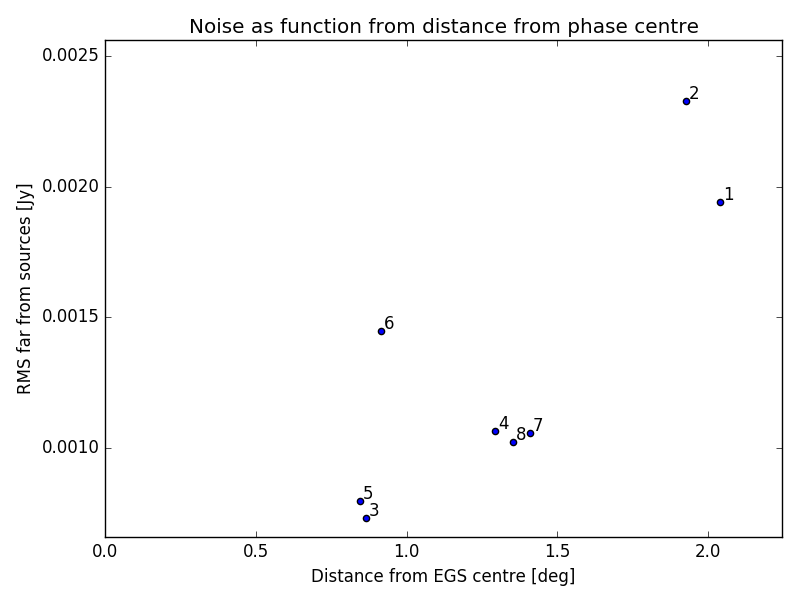
\includegraphics[width=0.8\linewidth]{images/RMSvsDistFromEGS.png}
\caption{Thermal noise near LBCS sources as a function of distance from the phase centre.}
\label{fig.noiserms.distEGS}
\end{figure}

\pg
To estimate the prevalence of directional gain errors, we then calculate the rms around each LBCS source. This is plotted in \cref{fig.dderms.distEGS}. The RMS around each source is normalised by the source's integrated flux as calculated on the restored image: this is because we expect brighter images to show stronger artefacts associated to directional gain errors. It should be noted that LBCS8 is not deconvolved at all: as such, its RMS is effectively calculated on a corrupted dirty map of the source, rather than a residual map. This helps explains its outlier behaviour. This outlier aside, the directional gain rms seems fairly flat as a function of distance from 3C295, however - a very good sign, as it indicates that the directional gain errors are comparable across the primary beam. However, we do not take into account the increase in thermal rms as a function of distance from phase centre in this plot. We therefore look at the normalised RMS values for each LBCS source, shown in \cref{fig.rmsratio.distEGS}. Here the relationship becomes even flatter, though LBCS5 now stands as a $3\sigma$ outlier. The blue line shows the mean value, excluding LBCS8; it lies at $y=1.08063981$. In other words, the average RMS induced by directional gain errors, when normalised by both the flux of a source for which it is calculated and the thermal noise, is very close to unity, and does not increase very much as distance from 3C295 increases. While it apparently increases in the direction of LBCS5, the EGS is not in this direction from 3C295, and so this is not a source of concern for our project of imaging the EGS using international LOFAR.
\begin{figure}[h!]
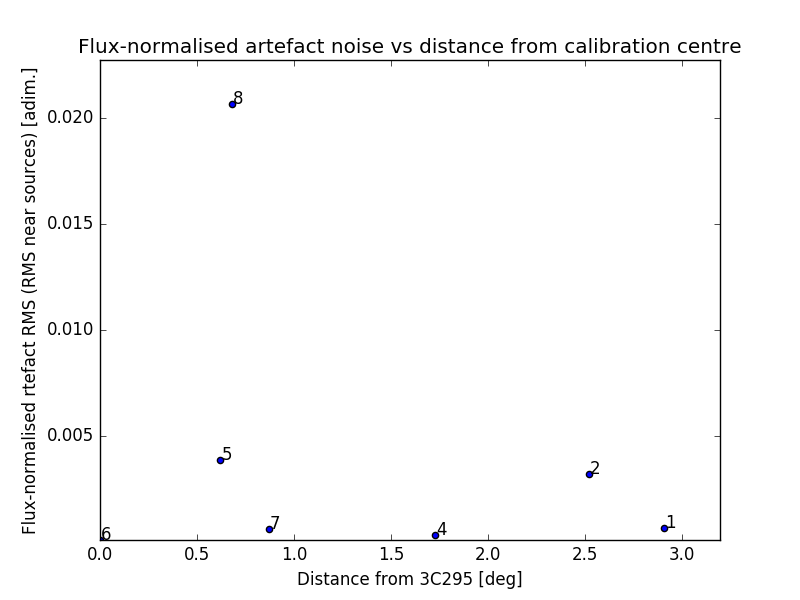
\includegraphics[width=0.8\linewidth]{images/ArtefactRMSvsDistFrom3c295.png}
\caption{DDE noise near LBCS sources as a function of distance from the phase centre. Because 3C295 is so much brighter than all other sources ($\sim100$Jy; second-brightest LBCS source is $\sim2$Jy), its DDE noise was normalised by its integrated model flux.}
\label{fig.dderms.distEGS}
\end{figure}
\begin{figure}[h!]
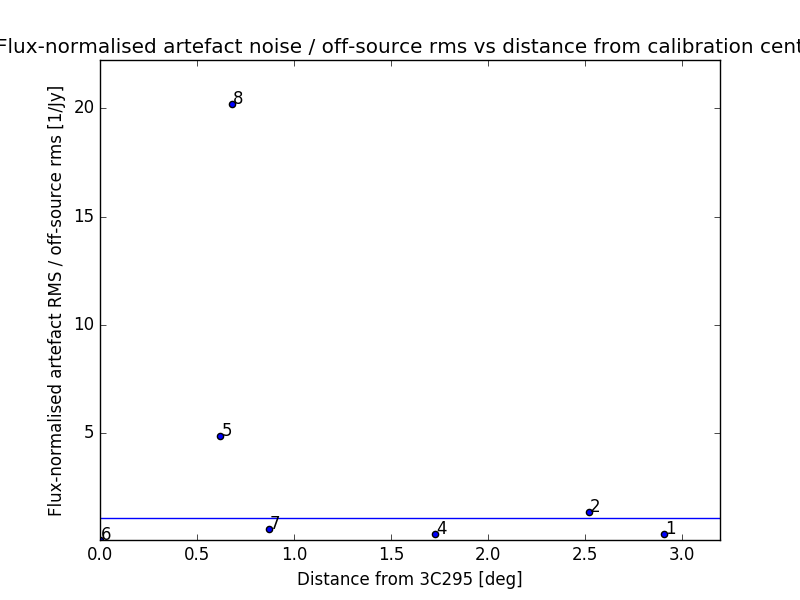
\includegraphics[width=0.8\linewidth]{images/NormArtefactRMSvsDistFrom3c295.png}
\caption{}
\label{fig.rmsratio.distEGS}
\end{figure}

\pg
\textcolor{red}{need LBCS3 to finish imaging to really conclude here, sadly. the EGS lies in a triangle between 3C295, LBCS4 and LBCS3 , so if LBCS3 is fine, then the project is fine!}



\clearpage
\section{Patchwise Imaging of the EGS using LOFAR International Stations}

\pg
\textcolor{red}{check that nancep3 can be used for another week and talk about source subtraction; if project cannot go ahead in the next 2 weeks (which it should be able to if we don't self-cal) then scrap this section and move straight on to conclusions \& future work.}



